\documentclass[11pt,a4paper]{article}
\usepackage[margin=22mm]{geometry}
\usepackage[T1]{fontenc}
\usepackage[utf8]{inputenc}
\usepackage{lmodern,amsmath,amssymb,booktabs,longtable,graphicx,xcolor,hyperref,array}
\hypersetup{colorlinks=true,linkcolor=blue,urlcolor=blue}
\setlength{\parskip}{6pt}
\setlength{\parindent}{0pt}
\renewcommand{\arraystretch}{1.15}
\begin{document}
\begin{center}
{\LARGE\bfseries ME2 - VCM on Raspberry Pi 5\\[5pt]}
{\large Two-stage, from-scratch voice command model}\par
Crizepvill F. Dumalaog \quad AI 231 Machine Exercise 2 \quad 1 October 2026
\end{center}

\begin{abstract}
This report documents the current training artifacts and code, including measured limits. A binary 2-class wake detector continuously evaluates local audio, then a 31-class intent classifier maps an accepted command to a coded action. Both use the same TinyDSCNN-48 topology and a 40-band log-mel frontend. Weather uses a separate live API; recognition itself uses no cloud model. The staged INT8 pair totals \textbf{76740 bytes}. The 95\% per-class goal is assessed on a reused speaker-held-out command set and is not assumed to be met.
\end{abstract}

\section{Requirements and command mapping}
The course asks for common smart-device interactions, multi-speaker speech, scratch training, a tiny offline classifier, and a Raspberry Pi demonstration. The class dataset contains 17986 command WAV rows from 100 reference speaker IDs. The 31 output labels refine the ten requested command families into fixed slot values. The wake phrase is a separate binary output, not a 32nd intent class.

\small
\begin{longtable}{p{0.24\textwidth}>{\raggedright\arraybackslash}p{0.70\textwidth}}
\toprule Course command family & Dataset labels \\
\midrule\endhead
Play music & PLAY\_MUSIC \\
Questions: weather and time & WEATHER, TIME \\
Lights on and off & LIGHT\_ON, LIGHT\_OFF \\
Brightness and color & BRIGHTNESS\_20, BRIGHTNESS\_60, BRIGHTNESS\_100, COLOR\_RED, COLOR\_GREEN, COLOR\_BLUE \\
Timers & TIMER\_10s, TIMER\_30s, TIMER\_1m \\
Alarms & ALARM\_6\_00AM, ALARM\_8\_00AM, ALARM\_9\_00PM \\
Thermostat setpoints & TEMPERATURE\_18, TEMPERATURE\_22, TEMPERATURE\_26 \\
Media and volume & PAUSE, STOP, NEXT, VOLUME\_UP, VOLUME\_DOWN \\
Reminders and lists & LIST\_REMINDERS,\newline CREATE\_REMINDER\_DRINK\_WATER,\newline CREATE\_REMINDER\_EXERCISE,\newline CREATE\_REMINDER\_STUDY \\
Calls and messaging & CALL, MESSAGE \\
\bottomrule
\end{longtable}
\normalsize

The recorder's 31 intent choices match the model label order and manifest labels. Each suggested phrase is the most frequent exact transcript for its class and is stored in a per-label text file; new takes also save the displayed prompt in the \texttt{suggested\_phrase} manifest column. This field stores the prompt, not an automatic transcript. Earlier 936 rows have no recoverable prompt or transcript and remain blank. For \texttt{LIGHT\_OFF}, the current suggestion is \emph{Kill the lights}, the most frequent matching training transcript (200 clips). Four additional recorder choices are \texttt{wake\_word}, \texttt{\_unknown\_}, \texttt{\_background\_noise\_}, and \texttt{\_silence\_}. Exact legacy command mappings are accepted; unsupported old slot values stay excluded. The machine-readable check is \path{docs/ME2_DATASET_ALIGNMENT.json}.

\section{Data provenance and split discipline}
The dataset's local README attributes its reference voices to LibriSpeech and SilencioPH. The manifest uses 14370 train, 1818 validation, and 1798 test rows, with reference speakers separated by partition. WAVs are read and resampled to 16 kHz by the frontend when necessary. The current human recorder manifest has 936 rows from three anonymous IDs, dominated by person-01; exact waveform deduplication leaves 699 eligible single-label PCM groups, with one cross-label collision excluded while both original files remain. The staged 2026-09-30 pair was trained on the earlier 851-row snapshot (614 groups). The 2026-10-01 candidate uses 374 eligible personal training clips plus the reference training split. All 31 intent classes have mapped personal examples, but amounts and acoustic conditions remain uneven. The personal split is by deduplicated waveform within label, so speakers can occur in training and test. These personal scores are \emph{not} unseen-speaker evidence.

The wake optimizer labels every command in the reference \emph{training} partition as \texttt{NON\_WAKE}, along with training-only personal commands, unrelated speech, room noise and silence. The positive class is the recorded wake phrase. Validation and test partitions are not optimization inputs. Class weighting counters the large negative-to-positive imbalance. The intent optimizer uses the 31-class reference training partition and exact-mapped personal training takes. No pretrained weights or ASR model are loaded.

\section{Signal path and architecture}
Capture is mono at 16 kHz. A 2.5 s window contains 40,000 samples. The frontend computes a 512-point short-time Fourier transform using a 400-sample Hann window and 160-sample hop, projects power to 40 mel bands, applies log compression, then standardizes the feature tensor. The resulting network input is $(1,40,251)$ per item. The 25 ms window, 10 ms hop, and FFT size are distinct quantities; the 512-point transform zero-pads each 400-sample analysis frame.

\begin{figure}[htbp]\centering
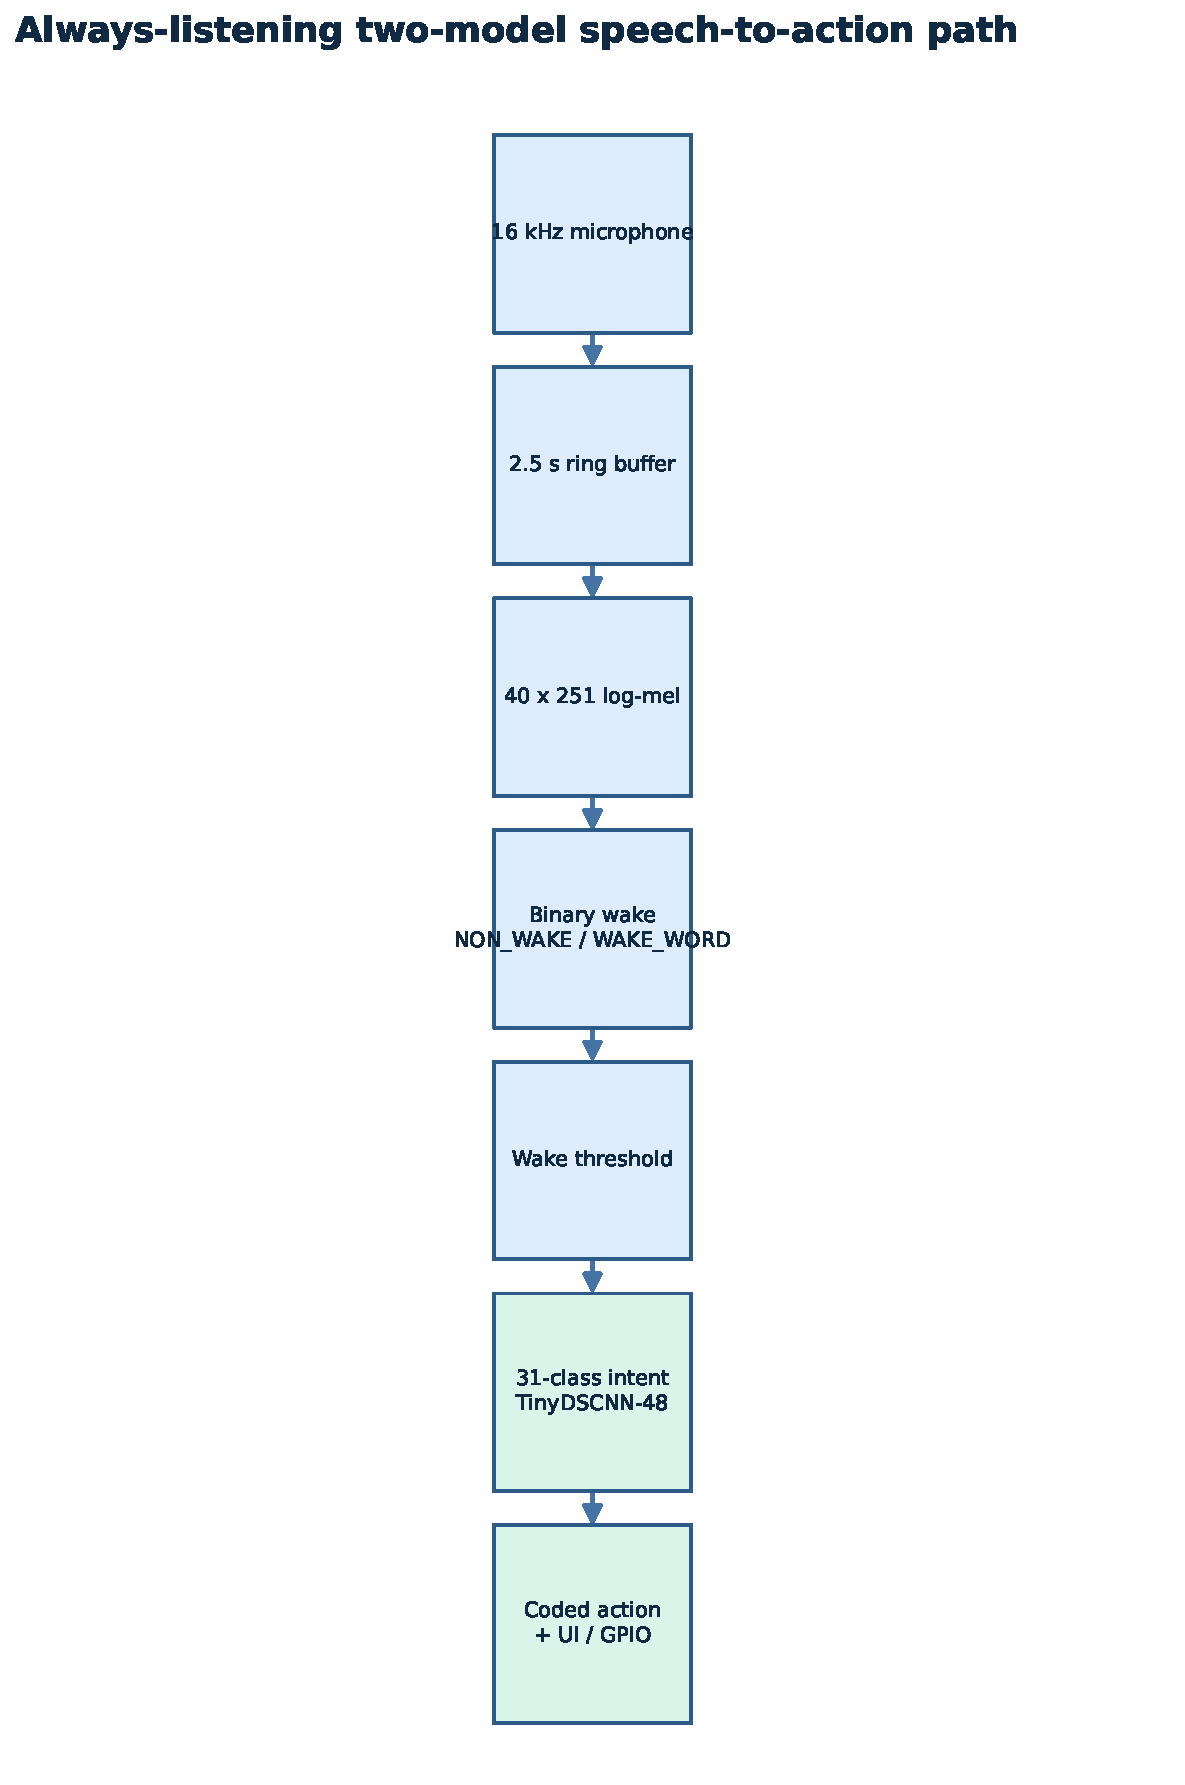
\includegraphics[height=0.70\textheight,keepaspectratio]{ME2_two_stage_connections.pdf}
\caption{The actual two-model routing. The wake gate precedes intent inference; actions are coded, not generated by an LLM.}
\end{figure}

The stem is a $5\times5$ convolution with stride $(2,2)$, 48 output channels, batch normalization and ReLU. Four depthwise-separable blocks each contain a $3\times3$ channel-wise convolution, batch normalization, ReLU, a $1\times1$ pointwise convolution, batch normalization and ReLU. Block 2 halves the time dimension. Global average pooling yields 48 features, followed by dropout $p=0.15$ during training and a linear head. Only that head differs between the two models.

\begin{longtable}{p{0.48\textwidth}p{0.28\textwidth}r}
\toprule Stage & Output $(C,F,T)$ or vector & Parameters \\
\midrule\endhead
Input log-mel & (1, 40, 251) & 0 \\
5x5 stem / BN / ReLU & (48, 20, 126) & 1,296 \\
DS block 1 & (48, 20, 126) & 2,928 \\
DS block 2 & (48, 20, 63) & 2,928 \\
DS block 3 & (48, 20, 63) & 2,928 \\
DS block 4 & (48, 20, 63) & 2,928 \\
Global average pool & (48,) & 0 \\
Linear head: 31 logits & (31,) & 1,519 \\
\midrule \textbf{Intent total} & \textbf{31 logits} & \textbf{14,527} \\
\textbf{Wake total} & \textbf{2 logits} & \textbf{13,106} \\
\bottomrule\end{longtable}

\begin{figure}[htbp]\centering
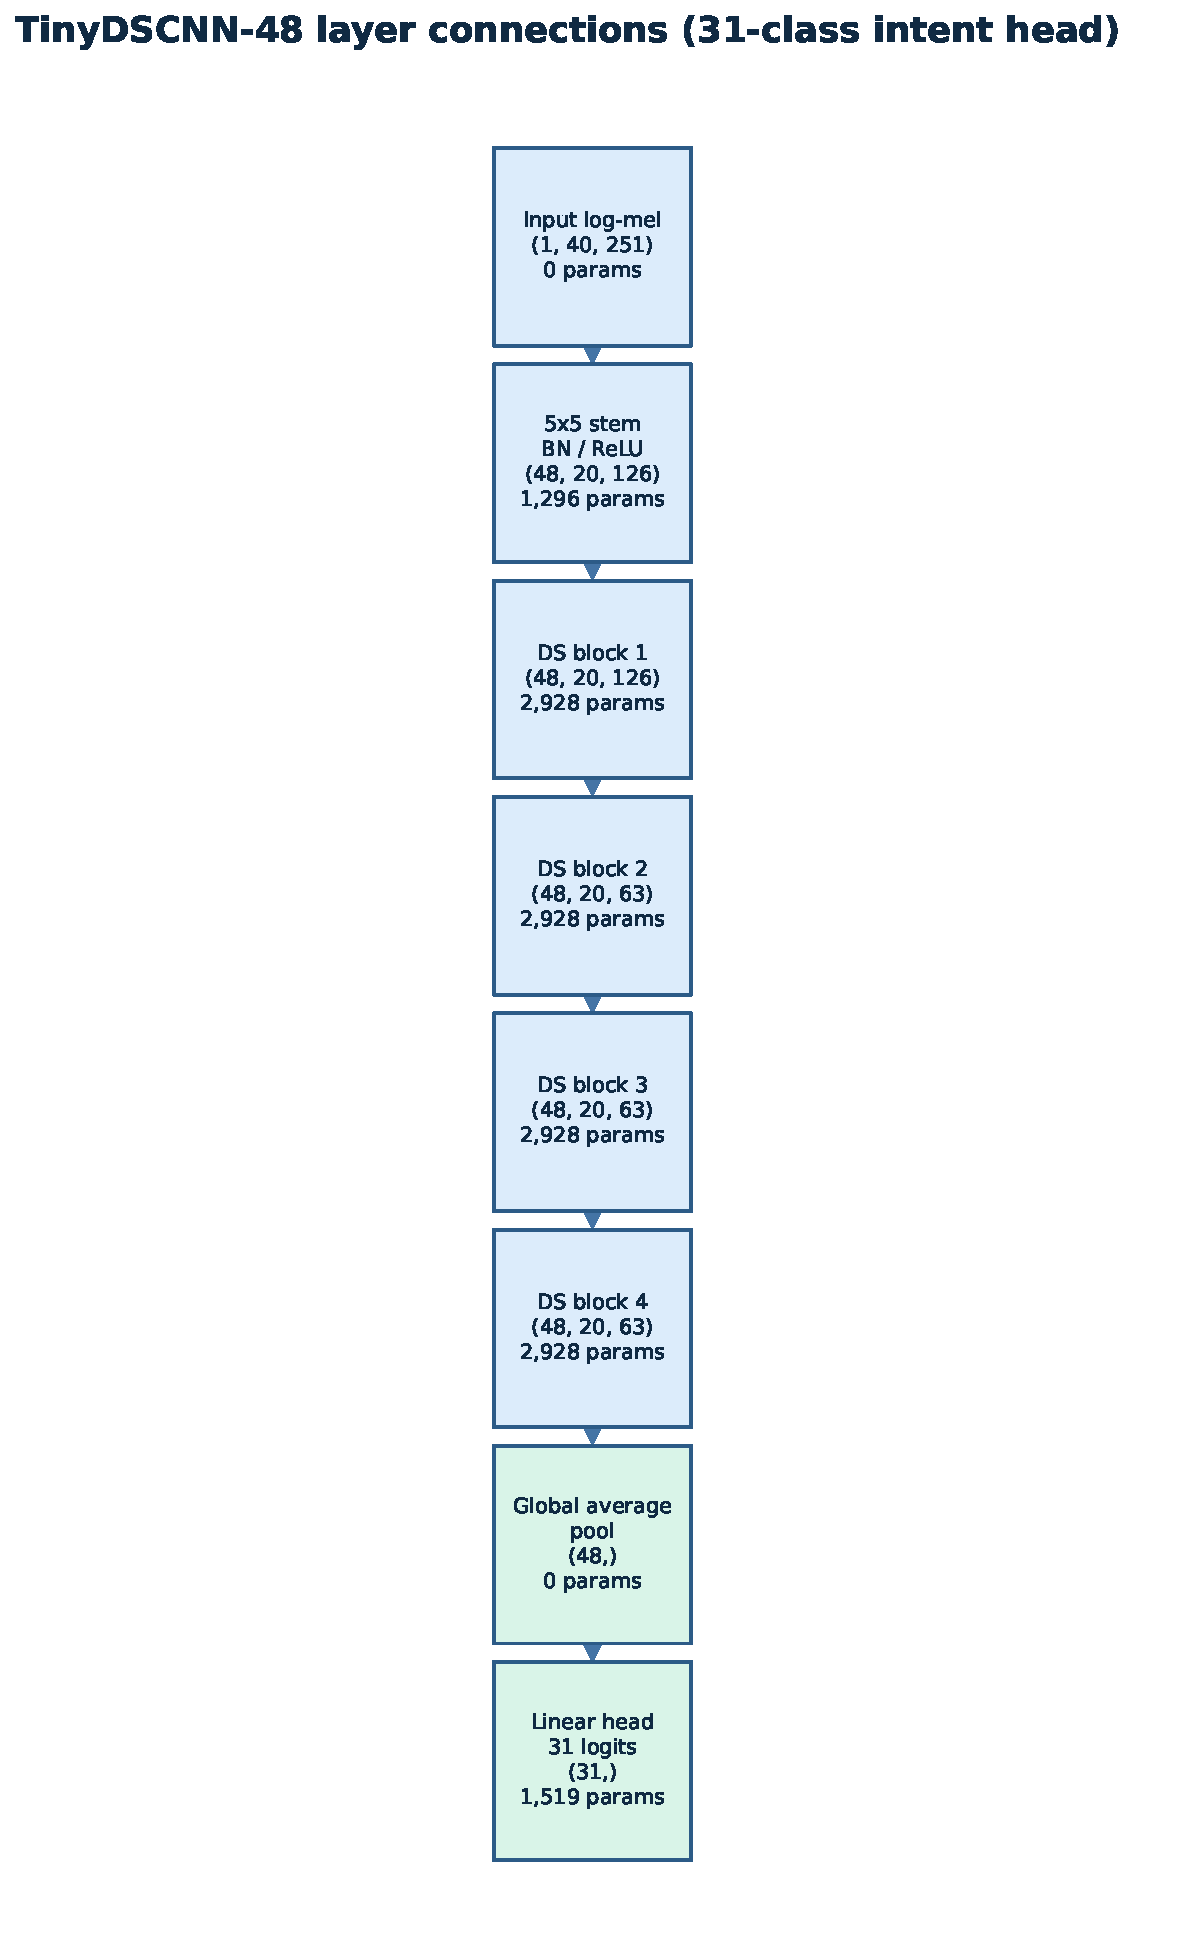
\includegraphics[height=0.72\textheight,keepaspectratio]{ME2_TinyDSCNN48_connections.pdf}
\caption{Layer-stage connections drawn with NetworkX from a live PyTorch shape and parameter inspection.}
\end{figure}

For 48 input and output channels, a conventional $3\times3$ convolution has $9\cdot48^2=20,736$ kernel weights. Each depthwise/pointwise pair has $9\cdot48+48^2=2,736$ kernel weights, before normalization parameters: about $7.58$ times fewer convolution weights. The full heads contain 13,106 and 14,527 parameters. Static QDQ INT8 ONNX export uses training-only calibration features.

\section{Training and measurements}
Two from-scratch pairs are retained for comparison. The staged/Pi pair is \texttt{me2-vcm-20260930-human851}: binary wake used seed 231 for 30 epochs; 31-class intent used seed 232 for 60 epochs and mixed 315 deduplicated personal training clips with 14370 reference training clips. The latest unpromoted candidate is \texttt{me2-vcm-20261001-human936}; it was trained from random initialization with the same epoch counts and seeds, using the current eligible personal corpus. AdamW with cosine learning-rate decay optimized both models; time/frequency masks and limited temporal jitter augmented training. Checkpoints and wake calibration used validation data. The reference test partition has been used in prior iterations, so these scores are comparisons on a reused benchmark, not a pristine one-time test.

The staged wake model uses a fixed 0.95 probability cutoff. Its saved-clip replay accepted \textbf{8/8} held-out personal wake clips, falsely accepted \textbf{0/120} personal non-wake clips, and falsely accepted \textbf{0/1798} reference commands. The new candidate selected a 0.999827 INT8 threshold on validation and accepted \textbf{6/8} held-out personal wake clips, with \textbf{0/134} personal non-wake and \textbf{0/1798} reference-command false accepts. Only eight positives were held out, so the candidate calibration is unstable. Neither replay measures continuous false activations per hour.

The staged INT8 intent classifier reached \textbf{97.22\% accuracy} and \textbf{97.22\% macro F1} on 1798 reused reference test clips. On its earlier 101-clip personal test it reached \textbf{92.08\% accuracy} and \textbf{93.62\% macro F1}. The new candidate scored \textbf{96.89\% accuracy} / \textbf{96.90\% macro F1} on the same reused reference partition and \textbf{92.17\% accuracy} / \textbf{92.44\% macro F1} on a different 115-clip personal split. Candidate reference F1 is below 95\% for \texttt{BRIGHTNESS\_100}, \texttt{BRIGHTNESS\_20}, \texttt{TEMPERATURE\_18}, \texttt{TEMPERATURE\_22}, and \texttt{TIME}. Candidate personal F1 is below 95\% for \texttt{ALARM\_6\_00AM}, \texttt{ALARM\_8\_00AM}, \texttt{BRIGHTNESS\_100}, \texttt{BRIGHTNESS\_20}, \texttt{COLOR\_RED}, \texttt{LIGHT\_OFF}, \texttt{LIST\_REMINDERS}, \texttt{MESSAGE}, \texttt{NEXT}, \texttt{PAUSE}, \texttt{PLAY\_MUSIC}, and \texttt{VOLUME\_UP}. The goal of at least 95\% F1 for every class is not met. Personal scores have small support and share speakers across training and test. On the candidate personal test rows, intent replay got red 2/3, green 3/3, blue 3/3, and \texttt{LIGHT\_OFF} 3/5; the off mistakes mapped to \texttt{MESSAGE} and \texttt{ALARM\_8\_00AM}. The staged model got 3/3 on each color and 4/5 off on these same rows, but its older training data may overlap them, so this comparison is diagnostic rather than a clean paired test. The code-level simulated RGB actions return the expected red, green, blue, and off output states. A 0.95 intent-confidence rejection cutoff retained only 2/14 tested color/off clips; confidence cutoff is not an accuracy guarantee and is not configured. Full candidate metrics appear in \path{docs/evaluations/phrase-prompt-class-metrics-20261001.csv}.

\footnotesize
\begin{longtable}{p{0.34\textwidth}rrrrr}
\toprule Intent class & Staged ref F1 & Recall & n & Staged personal F1 & n \\
\midrule\endhead
ALARM\_6\_00AM & 99.1 & 98.3 & 58 & 100.0 & 2 \\
ALARM\_8\_00AM & 99.1 & 100.0 & 56 & 80.0 & 2 \\
ALARM\_9\_00PM & 100.0 & 100.0 & 58 & 100.0 & 3 \\
BRIGHTNESS\_100 & 96.8 & 100.0 & 60 & 100.0 & 4 \\
BRIGHTNESS\_20 & 97.5 & 98.3 & 60 & 100.0 & 3 \\
BRIGHTNESS\_60 & 98.3 & 96.7 & 60 & 100.0 & 3 \\
CALL & 97.2 & 96.3 & 54 & 66.7 & 2 \\
COLOR\_BLUE & 94.0 & 91.7 & 60 & 100.0 & 3 \\
COLOR\_GREEN & 98.3 & 96.7 & 60 & 100.0 & 3 \\
COLOR\_RED & 94.5 & 100.0 & 60 & 100.0 & 3 \\
CREATE\_\allowbreak REMINDER\_\allowbreak DRINK\_\allowbreak WATER & 97.6 & 100.0 & 60 & 100.0 & 3 \\
CREATE\_\allowbreak REMINDER\_\allowbreak EXERCISE & 99.2 & 98.3 & 60 & 100.0 & 3 \\
CREATE\_\allowbreak REMINDER\_\allowbreak STUDY & 99.2 & 98.3 & 60 & 100.0 & 3 \\
LIGHT\_OFF & 94.3 & 96.7 & 60 & 80.0 & 5 \\
LIGHT\_ON & 95.2 & 92.6 & 54 & 100.0 & 4 \\
LIST\_REMINDERS & 94.7 & 93.1 & 58 & 100.0 & 2 \\
MESSAGE & 97.3 & 94.8 & 58 & 100.0 & 3 \\
NEXT & 99.2 & 98.3 & 60 & 66.7 & 2 \\
PAUSE & 98.2 & 98.2 & 56 & 61.5 & 9 \\
PLAY\_MUSIC & 98.3 & 100.0 & 58 & 61.5 & 4 \\
STOP & 94.5 & 96.3 & 54 & 100.0 & 7 \\
TEMPERATURE\_18 & 95.7 & 93.3 & 60 & 100.0 & 3 \\
TEMPERATURE\_22 & 96.0 & 100.0 & 60 & 100.0 & 4 \\
TEMPERATURE\_26 & 98.3 & 96.7 & 60 & 100.0 & 3 \\
TIME & 95.1 & 90.7 & 54 & 85.7 & 3 \\
TIMER\_10s & 95.0 & 95.0 & 60 & 100.0 & 3 \\
TIMER\_1m & 99.1 & 100.0 & 56 & 100.0 & 3 \\
TIMER\_30s & 96.6 & 95.0 & 60 & 100.0 & 3 \\
VOLUME\_DOWN & 98.1 & 100.0 & 52 & 100.0 & 3 \\
VOLUME\_UP & 99.2 & 98.3 & 60 & 100.0 & 1 \\
WEATHER & 98.1 & 100.0 & 52 & 100.0 & 2 \\
\bottomrule\end{longtable}
\normalsize
\normalsize

\section{Runtime, controls, and hardware}
In standby, only the binary wake model runs after an energy gate. After wake, the intent model runs on the utterance. The ten-second command deadline now expires even if unrelated sound or pending speech persists. The Assistant and Studio both show the RGB light state. The device module implements fixed light levels/colors, playback/next/pause/stop, timer/alarm state, and temperature setpoints. A local generated melody provides deterministic music for an offline demo. Calls and messages are explicitly simulations; no telephony API is connected.

Weather is fetched asynchronously from the Open-Meteo current-weather API when networking is available; no weather API key is required. A failure returns a clear unavailable message without blocking microphone inference. Recognition remains local. The UI can change its capture microphone without reloading models; it retries after disconnects. Browser audio output selection uses \texttt{setSinkId} where supported. One cached browser speech voice is used consistently, and its volume follows the slider; the Pi also adjusts the ALSA mixer when available. A separate Restart VCM control remains for full service recovery. The recorder now exposes an immediate \textbf{Record again} control after saving.

\section{Raspberry Pi deployment and remaining gates}
The staged Pi release is \path{dandan-vcm-20260930.zip}, last verified under \path{/home/dalmacio/Desktop/dandan}. It is an application package, not an SD-card image. It includes both INT8 ONNX models, hashes, the frontend, action code, local demo music, an executable manual \path{launch-vcm.sh}, and an on-device verifier. It does not enable boot autostart. On ARM64, the last verified frontend-plus-model $p_{95}$ was 5.602 ms for wake and 5.453 ms for intent. The Pi PCM mixer responded to a 35\% volume request and was restored to 100\%. Earlier GPIO red/green/blue/off checks passed. The Pi last reported no capture device, so live speech remains untested. On 1 October 2026, SSH timed out and the local tunnel was absent; physical LEDs and current Pi service state could not be rechecked. The existing \path{/home/dalmacio/vcm} project was left untouched. Windows users can launch the Pi and open the tunneled Assistant by double-clicking \path{C:/Users/danda/Desktop/dandan/Start-VCM.bat} after network access returns.

For a class demonstration, show the wake transition first, then light brightness/color, volume, local music, temperature, and weather. State plainly that the RGB panel and thermostat are simulations unless GPIO/HVAC hardware is connected. For a stronger performance claim, record multiple sessions and all 31 classes from additional speakers, hold complete speakers out, collect room noise and near-miss wake phrases, and measure continuous false activations per hour. Create a fresh sealed test set for the next evaluation.

\end{document}
